\newpage
\section{A Moving Image}

In this activity, we are going to explore how reflections are related
to translations.  Consider the following ``F'' shape:
\[
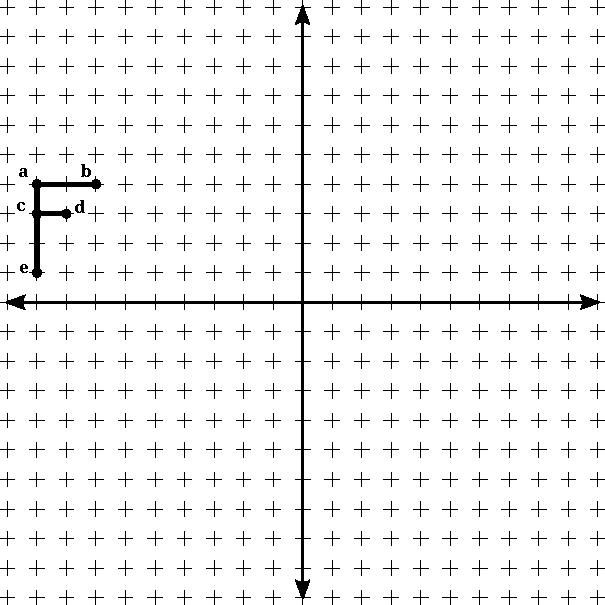
\includegraphics{../graphics/planeF.pdf}
\]

\begin{prob}
Use two reflections to translate the ``F'' shape 8 units to the
right. Don't worry about the actual matrices involved.
\end{prob}

\begin{prob}
What reflections would translate the original ``F'' shape 4 units to
the right? Again, don't worry about the actual matrices involved.
\end{prob}

\begin{prob}
Can you generalize the two problems above? What composition of two
reflections will give a horizontal translation of $n$ units to the
right?
\end{prob}

\begin{prob} 
Now suppose you wish to move the original ``F'' shape 4 units to the
right, but you will first reflect via this matrix:
\[
\mat{F}_{x=0}  = 
\begin{bmatrix}
-1 & 0 & 0 \\
0 & 1 & 0 \\
0 & 0 & 1
\end{bmatrix}
\]
What is the other matrix that is needed?
\end{prob}

\begin{prob}
Generalize the problem above: Suppose you wish to translate the
original ``F'' shape $n$ units to the right, and you start by
reflecting by $\mat{F}_{x=0}$. What is the second matrix that you
apply?
\[
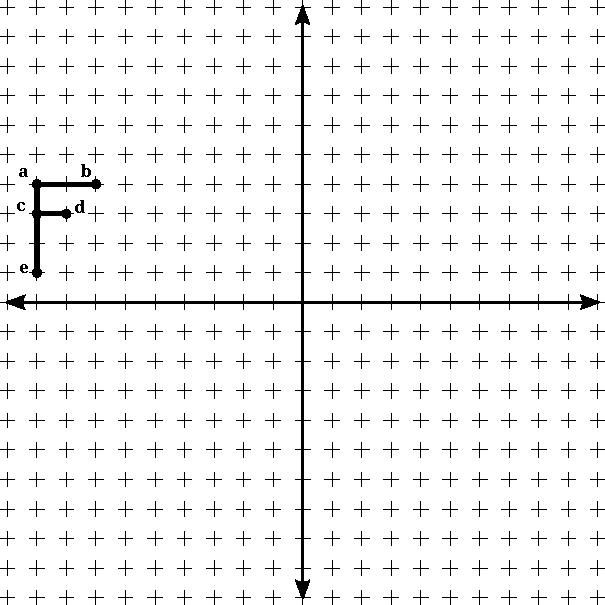
\includegraphics{../graphics/planeF.pdf}
\]
\end{prob}
